% \documentclass[]{article}
% \documentclass[letterpaper]{article}
% \setlength{\textwidth}{12cm}

% \usepackage[
% backend=biber,
% style=alphabetic,
% ]{biblatex}
\documentclass[letterpaper]{llncs}
\usepackage[letterpaper, margin=1.3in]{geometry}

\usepackage{mathpartir}
\usepackage{hyperref}
\usepackage{mathtools}
\usepackage{amsmath}
\usepackage{nccmath}
\usepackage{stmaryrd}
\usepackage{amssymb}
\usepackage{listings}


\usepackage{graphicx}
\graphicspath{ {./images/} }

\usepackage{url}

\makeatletter % allow us to mention @-commands
\def\arcr{\@arraycr}
\makeatother

\lstset{
    % identifierstyle=\color{violet},
    % textcolor=blue,
    % keywordstyle=\color{blue},
    keywordstyle=\text,
    basicstyle=\ttfamily,
    mathescape=true,
    showspaces=false,
    morekeywords={let, fix, in}
}
\usepackage[utf8]{inputenc}
% \usepackage[T1]{fontenc}


\title{Towards synthesis of stochastic programs from data}
\author{Thomas Logan}
\institute{University of Texas at Austin}

\begin{document}
\pagestyle{plain}

\maketitle

\section{Introduction}
This project aims to automate various portions of learning functions from data sets. 
The intended scenario consists of a user who wants to fit a line to some data
with some measure of uncertainty. To that end, this project attempts 
to simplify the notation for describing functions, and 
to remove the burden of specifying function shapes altogether. The first
part involves the compilation of programs followed by gradient descent, 
and the second parts involves the encoding of language followed by symbolic search. 

It is quite easy to describe an equation
from inputs to outputs in a typical programming language, such as the following:
\[ f(x) = m x + b \] 

However, current programming languages do not provide a compact notation 
for representing the requirement that the weights $m$ and $b$ are learned from data.
\textit{Pyro} \cite{pyro} is a language embedded in \textit{Python} \cite{python} for 
expressing the requirements of learning weights from data 
with probabilities for measuring uncertainty in the learned result. 
In Pyro, the simplest way to represent the above linear equation is as follows: 

\begin{lstlisting}[language=Python]
def model(xs, ys=None):
    m = pyro.param("m", torch.tensor(0.))
    b = pyro.param("b", torch.tensor(0.))
    
    with pyro.plate("data", len(xs)):
        return pyro.sample("ys", 
            dist.Normal(m * xs + b, 1.), obs=ys)
\end{lstlisting}

Clearly, there is a vast increase in notational noise, within which the essence of the idea is buried. 

To reduce the notational noise, this project introduces a simple programming language 
that allows expressing differentiable stochastic models in a succinct notation. In this new language,
we can express a model for learning a linear equation as follows: 

\begin{lstlisting}[language=Python]
x => {y | x, y : data}
    m $\sim$ normal(0., 1.); 
    b $\sim$ normal(0., 1.); 
    normal(m * x + b, 1)
\end{lstlisting}

The notation of our new language is is far more compact than Pyro's. 
It is only slightly more complicated than the bare linear equation, which is
due to annotating information about prior beliefs on the weights, the data, and 
distribution of the data in relation to the equation. 

Unfortunately, this solution leaves open another problem. How do we conjure up some 
initial belief about the distributions and the shape of the equation? 

To avoid needing to specify these details, we simplify the description further, such that the 
user can simply state the data and its relation to inputs and outputs. 

\begin{lstlisting}[language=Python]
x => {y | x, y : data}
\end{lstlisting}

The first part of the solution compiles a program of the DSL into a Pyro model and applies Pyro's 
\textit{stochastic variational inference} (SVI) algorithm \cite{svi} to learn posterior distributions for the weights. 

The second part of the solution encodes the DSL syntax and semantics into
a logical formula in Z3 \cite{z3} and uses Z3's \textit{satisfiability modulo theories} (SMT) technique \cite{smt} to search
for a program.  
The particular technique for constructing the search space from the syntax and semantics 
is based on that of Ellis et al \cite{ellis}.
Unfortunately, as of this writing, Z3 does not terminate in a reasonable amount of time\footnote{
I did a sanity check by removing most of the complex constraints to see if it could synthesize $x + y$.
It can if the constraints are specified in a particular (seemingly arbitrary way), but hangs forever
if the structure of the constraints is changed just slightly, 
such as introducing an intermediate variable, or changing the order of constraints.
}, 
despite using an encoding very similar to that of Ellis et al. 
After finding the program, the first part may be used to learn posteriors. 

\section{Language}

The programs in the domain specific language are constructed using the following syntax:

\[
  \begin{array}{l @{} l}
    f &{} ::= p \Rightarrow s\ b \\
    s &{} ::= \{ x \ |\ p : \text{data} \} \\
    p &{} ::= x  \ |\ x,\ p \\
    b &{} ::= x\ \sim\ d\ ;\ b \ |\ x\ \#\ n\ \sim\ d\ ;\ b \ |\ d \\ 
    d &{} ::= 
        \text{normal}(e, e) \ |\ 
        \text{lognorm}(e, e) \ |\ 
        \text{uniform}(e, e) \ |\ 
        \text{halfnorm}(e) \ |\ 
        @(e) \\ 
    e &{} ::= q\ \vec{r} \\
    r &{} ::= +\ q \ |\ -\ q \\
    q &{} ::= a\ \vec{z} \\
    z &{} ::= *\ q \ |\ /\ q \\
    a &{} ::= (e) \ |\ \text{mean}(x) \ |\ \text{align}(x)\\
  \end{array}
\]

To see what these combinations of syntax mean, consider a program
for predicting the number of unemployment insurance claims 
between after the 2008 recession and before the 2020 pandemic \cite{plot}.
Let's examine the plot of the data in Fig. \ref{fig:plot} to gauge its shape.
\begin{figure}[h]
\begin{center}
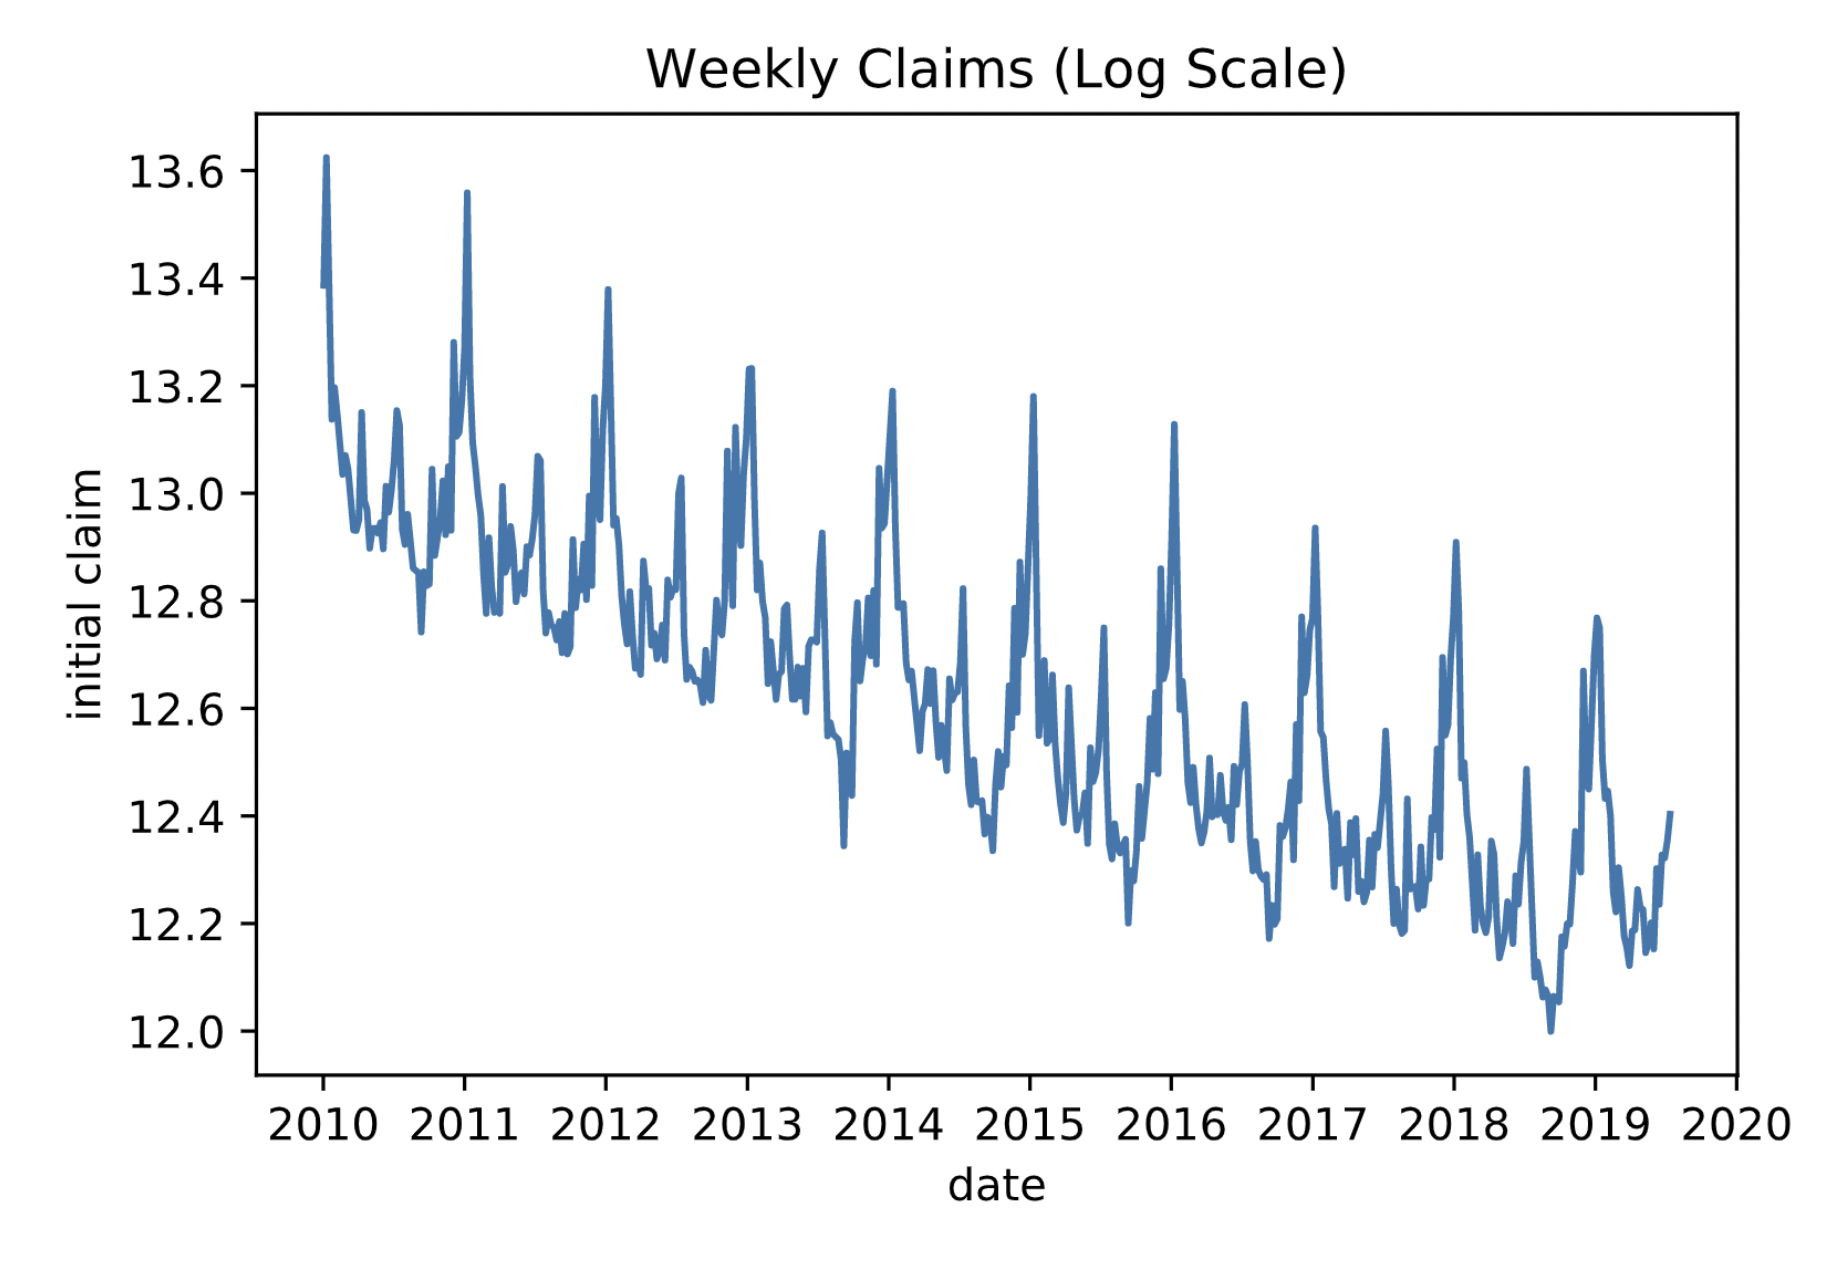
\includegraphics[scale=0.35]{weekly_claims}
\end{center}

\caption{
Weekly unemployment insurance claims. Source: Martin Jankowiak's slides \cite{plot}.   
}
\label{fig:plot}
\end{figure}
There appears to be an overall trend that's fairly linear with respect to the year. 
However, there are also periodic trends that seem to depend on the time of year.  
We can capture these trends with the following program:

\begin{lstlisting}[language=Python]
t => {n | t, n : data}
    m $\sim$ normal(0., 1.); 
    osd $\sim$ halfnorm(1.); 
    bs $\#$ 52 $\sim$ normal(0., 1.); 
    bs $\sim$ @(bs - mean(bs));
    lognorm(m * t + align(bs), osd)
\end{lstlisting}

The program represents a point-wise function from a weekly time index to a number of claims.
The parameter $t$ represents a single input. The variable $n$ represents
the ouput, such that the first column of the data are used as inputs, 
and second column of the data are observed outputs.
The rest of the program is the body of the function.
First, it samples a slope $m$ from a normal distribution centered at 0 with 
a standard deviation of 1. To handle the periodic trends, it constructs
a plate $bs$ of 52 independent elements, where each is sampled from 
a normal distribution. In order to ensure the weight $m$ governs
the overall trend, we need the values of $bs$ to cancel each other out.
To this end, the program recomputes the values of the plate vector point-wise 
by subtracting the mean from the original value. The notation $@$ simply indicates
to use the value of the expression directly.
The resulting number of claims is drawn from a log normal distribution
governed by $m * t + \text{align}(bs)$. The term $\text{align}(bs)$ takes an element from $bs$ 
at an implicit iteration index modulo 52. 



\section{Compiling programs into Pyro}
In order to learn the posterior distributions of our programs, the system compiles a program into  
a Pyro model and runs Pyro's SVI algorithm. For the most part, the compilation technique
is fairly standard, but the $\text{align}(\cdot)$ operator deserves special attention. 
Pyro's model operates over tensors of data, while the program DSL operates over points. 
This difference becomes noticeable when compiling the align operation. Tensor operations 
rely on data-parallelism. There is no
equivalent data-parallel operation for indexing a matrix with a vector of indices.
Thus, $\text{align}(\cdot)$ is actually compiled into repeating the target plate until it
to matches the size of the implicit number of total iterations.    
The example of unemployment insurance claims above is compiled into the following model.

\begin{lstlisting}[language=Python]
def model(t, n=None):
    m = pyro.sample("m", dist.Normal(0.0, 1.0))
    osd = pyro.sample("osd", dist.HalfNormal(1.0))
    with pyro.plate("bs_plate", 52):
        bs = pyro.sample("bs", dist.Normal(0.0, 1.0))
    bs = bs - bs.mean()
    with pyro.plate("data", len(t)):
        return pyro.sample("n", dist.Normal(
            m * t + bs.repeat(math.ceil(len(t)/len(bs)))
                [:len(t)], osd), obs=n)
\end{lstlisting}


\section{Encoding language into Z3}
In order to search for viable programs, the system encodes the language's syntax and semantics, 
along with the input data into a Z3 formula and runs Z3's SMT algorithm.
The technique for encoding a space of programs is far more intricate than compiling a program.
The technique used in this system is based on that of Ellis et al \cite{ellis}.

It constructs a search space recursively by following the structure of the syntax. 
If the syntax allows a choice of productions, it constructs a boolean control variable for each choice
and constructs an if-then-else term across each choice's abstract value, guarded with its respective control variable. 
The abstract value can be broken into two parts: a column\footnote{
To illustrate the concept of propagating Z3 terms we assume there's just one column.
In actuality, due to the plate concept, we have two columns: 
one for the mean and one for the align values of the plate.  
} of Z3 terms (one term per instance in the dataset) and a constraint.

For example, consider the part of the syntax for constructing the notions of sampling and distributions:

\[
  \begin{array}{l @{} l}
    b &{} ::= x\ \sim\ d\ ;\ b \ |\ x\ \#\ n\ \sim\ d\ ;\ b \ |\ d \\ 
    d &{} ::= 
        \text{normal}(e, e) \ |\ 
        \text{lognorm}(e, e) \ |\ 
        \text{uniform}(e, e) \ |\ 
        \text{halfnorm}(e) \ |\ 
        @(e) \\ 
  \end{array}
\]


This could generate the following column of terms in Z3:
\[
  \kappa_b[i] \triangleq
  \begin{array}[t]{l}
  \text{ite}(c_1, \llbracket \kappa_x[i]\ \sim\ \kappa_d[i]\ ;\ \kappa_b'[i]  \rrbracket, \\
    \hspace{4mm}\text{ite}(c_2, \llbracket \kappa_x[i]\ \#\ \kappa_n[i]\ \sim\ \kappa_d[i]\ ;\ \kappa_b'[i] \rrbracket, \\
        \hspace{8mm}\text{ite}(c_3, \llbracket \kappa_d[i] \rrbracket, \bot)))
  \end{array}
\]

Likewise, this could generate the following constraint in Z3:
\[
  \phi_b \triangleq
  \begin{array}[t]{l}
  \text{ite}(c_1, \llbracket \phi_x\ \sim\ \phi_d\ ;\ \phi_b'  \rrbracket, \\
    \hspace{4mm}\text{ite}(c_2, \llbracket \phi_x\ \#\ \phi_n\ \sim\ \phi_d\ ;\ \phi_b' \rrbracket, \\
        \hspace{8mm}\text{ite}(c_3, \llbracket \phi_d \rrbracket, \bot)))
  \end{array}
\]

It propagates description lengths for each subterm in a similar fashion.

Additionally, the system constructs the constraint such that at most one control variable for a particular set of choices    
is allowed to be true, which along with the if-then-else constraint, ensures
that exactly one subterm for each choice is identified, if there is a solution.  

\[
  \bigwedge\nolimits_i \bigwedge\nolimits_j (c_i = c_j) \vee \neg (c_i \wedge c_j) 
\]


The encoding specifies how leaf terms are denoted as Z3 formulas for each input instance.
The leaf syntax representing a parameter simply denotes a the corresponding column of the input data. 
The denotation may be abstract, consisting of both a Z3 term and a Z3 constraint on that term. 
The formulas of subterms are propagated up to larger composite terms according to the semantics of 
the composite terms.

Since the ultimate goal is to extract a program, the procedure also 
builds a tree with choices indexed by control variables, mirroring the Z3 formula.
Once a solution is found, the program can be extracted from the tree by selecting
the branches with a control variable that Z3 declared to be true.

The above mentioned portion of the syntax could lead to a search space tree that looks as follows:
\[
  \begin{array}{l }
    \{ \\
    \hspace{6mm} c_1 \mapsto x_1\ \sim\ \{ \\
        \hspace{12mm} c_4 \mapsto \text{normal}(\hdots), \\
        \hspace{12mm} c_5 \mapsto \text{lognorm}(\hdots), \\ 
        \hspace{12mm} \vdots \\
    \hspace{6mm}\},\\
    \hspace{6mm} c_2 \mapsto x_2\ \#\ n\ \sim\ \{ \\
        \hspace{12mm} c_9 \mapsto \text{normal}(\hdots), \\
        \hspace{12mm} c_{10} \mapsto \text{lognorm}(\hdots), \\ 
        \hspace{12mm} \vdots \\
    \hspace{6mm}\},\\
    \hspace{6mm} c_3 \mapsto \{ \\
        \hspace{12mm} c_{14} \mapsto \text{normal}(\hdots), \\
        \hspace{12mm} c_{15} \mapsto \text{lognorm}(\hdots), \\ 
        \hspace{12mm} \vdots \\
    \hspace{6mm}\}\\
    \}
    
  \end{array}
\]

To measure the correctness of a found program $f$, 
the synthesis procedure defines a cost in terms of a program's
description length $-\text{log}\ \text{L}(f)$ and its noise $-\text{log}\ \text{P}(y|f(x)) $.
A length is associated with each production rule in the syntax.
Summing together the length across all the nodes of a program results 
in a total description length for that program. 
Noise is defined as the distance between the expected and actual results.

\[
    - \text{log}\ \text{P}(y|f(x)) \triangleq |y - f(x)| 
\]

The total cost of a found program is the sum of the description length and the total noise over all the data. 
The system encodes this cost (or loss) definition in Z3.
\[
    \ell = - \text{log}\ \text{L}(f) + \sum_{i=1}^N - \text{log}\ \text{P}(y_i|f(x_i))
\]

The synthesis procedure asks Z3 to search the space for a program
and its cost. If Z3 finds a program and a cost, the procedure 
adds the constraint that the cost must be less than the cost just found
and asks Z3 to find another. This repeats until Z3 cannot find a solution.

\[
\begin{array}{l}
  \text{search}(\phi, \sigma) \triangleq \\
    \hspace{6mm}\begin{array}{@{} l}
    \text{match}\ \text{solve}(\phi) \\
    \cdot\ \bot \Rightarrow \sigma \\
    \cdot\ \sigma' \Rightarrow \text{search}(\phi \wedge (\ell < \sigma'[\ell]), \sigma')
      % \hspace{6mm}\begin{array}{@{} l}
      %   \text{match}\ spurious(\pi, \vec{e}) \\
      %   \cdot\ \bot \Rightarrow \pi\\
      %   \cdot\ proof \Rightarrow \text{search}(\vec{e}, \Omega \cup predicates(proof))
      % \end{array}
    \end{array}
\end{array}
\]

The last found program is the best solution. The procedure 
extracts the program by following the branches indicated by the 
control variables. 

There are a number of details of this language that require 
special attention and do not fit neatly into the framework  
developed by Ellis et al.
% Encoding plates: mean and align
Due to the concept of plates and its 
$\text{mean}(\cdot)$ and $\text{align}(\cdot)$ operators,
the encoding must actually propagate two columns of output formulas,
one for mean, and one for align. 
For non-plate terms that do not produce a plate, they simply
produce the mean column, and leave the align column empty.  

When generating plate distributions, it constructs a matrix of weight variables,
where the number of columns corresponds to the size of the plate, and the number of rows corresponds
to that of the data.
A plate's mean column is the mean across plate elements in each row. 
a plate's align column is the mean across instances in each column, rotated and realigned with number of instances. 

% Encoding distribution constraints
The encoding handles the semantics of distributions by introducing fresh weight variables  
and adding constraints over those variables representing a plausible range of values
within the distribution. For the normal distribution, it requires a lower bound of 
$\mu - 3 * \sigma$ and an upper bound of $\mu + 3 * \sigma$,
where $\mu$ is the center of the distribution, and $\sigma$ is the standard deviation.
For the log normal distribution, it uses the mode, mean, and skewness to define the boundaries
of plausible values. 

% Encoding with variables and plates in scope
Since the language allows assigning variables to expressions, it is necessary to keep track
of variable scoping and which columns of abstract values are associated with which variables. 
Thus, when generating expressions with variables, the encoding is limited to variables that
are in scope, and their associated abstract values are propagated.

\section{Conclusion}
This work has presented an initial solution to the problem of finding stochastic functions that fit data.
The first part simplifies describing functions with prior beliefs and data by defining a DSL for
point-wise functions that are implicitly indexed and compiling these simple representations
into more complicated Pyro models over tensors. It runs Pyro's SVI algorithm to learn the posterior weights. 
The second part removes the burden of describing the function body by encoding the language and data into a Z3 formula. 
It iteratively solves the formula and adds increasingly strict cost constraints to lower
the cost of the found function each iteration.  
The source code can be retrieved from \url{https://github.com/resin-studio/ballistic}.

\newpage

\begin{thebibliography}{9}

\bibitem{pyro}
E.Bingham, J.P. Chen, M. Jankowiak, F. Obermeyer, N. Pradhan, T.Karaletsos, R. Singh, P. Szerlip, P. Horsfall and, N.D. Goodman. Pyro: Deep universal probabilistic programming. In JMLR, 2019. 

\bibitem{python} 
G. Van Rossum, F.L. Drake. Introduction to python 3: python documentation manual part 1. In CreateSpace, 2009.

\bibitem{svi}
M.D. Hoffman, D.N. Blei, C. Wang, J. Paisley. Stochastic variational inference. In JMLR, 2013.

\bibitem{z3}
L. De Moura, N. Bjørner, Z3: An efficient SMT solver. In, TACAS, 2008. In ETAPS, 2008.

\bibitem{smt}
C. Barrett, R. Sebastiani, S. Seshia, C. Tinelli. Satisfiability Modulo Theories. In
Handbook of Satisfiability. IOS Press, 2009.

\bibitem{ellis}
K. Ellis K, A. Solar-Lezama A, J. Tenenbaum. Unsupervised learning by program synthesis. In NIPS, 2015.

\bibitem{plot}
M. Jankowiak. Retrieved 2023-4-28 from \url{http://docs.mlinpl.org/conference/2019/slides/martin_jankowiak_mlinpl2019.pdf} 


\end{thebibliography}

\end{document}